\documentclass[tikz,a4paper,11pt]{book}
%\documentclass[a4paper,twoside,11pt,titlepage]{book}
\usepackage{listings}
\usepackage[utf8]{inputenc}
\usepackage[spanish,es-noquoting]{babel}
\usepackage{forest}
\usepackage{adjustbox}
\usepackage{caption}
\usepackage{float}
\usetikzlibrary{arrows.meta,shapes,positioning,trees}

% \usepackage[style=list, number=none]{glossary} %
%\usepackage{titlesec}
%\usepackage{pailatino}

\decimalpoint
\usepackage{dcolumn}
\newcolumntype{.}{D{.}{\esperiod}{-1}}
\makeatletter
\addto\shorthandsspanish{\let\esperiod\es@period@code}
\makeatother


%\usepackage[chapter]{algorithm}
\RequirePackage{verbatim}
%\RequirePackage[Glenn]{fncychap}
\usepackage{fancyhdr}
\usepackage{graphicx}
\usepackage{afterpage}
\usepackage{longtable}
\usepackage[pdfborder={000}]{hyperref} %referencia

% ********************************************************************
% Re-usable information
% ********************************************************************
\newcommand{\myTitle}{Synapse Messenger\xspace}
\newcommand{\myDegree}{Grado en Ingeniería Informática\xspace}
\newcommand{\myName}{Marco Manuel Fernández Pranno\xspace}
\newcommand{\myProf}{Juan Julián Merelo Guervós\xspace}
\newcommand{\myFaculty}{Escuela Técnica Superior de Ingenierías Informática y de Telecomunicación\xspace}
\newcommand{\myFacultyShort}{E.T.S. de Ingenierías Informática y de Telecomunicación\xspace}
\newcommand{\myDepartment}{Departamento de Arquitectura y Tecnología de Computadores\xspace}
\newcommand{\myUni}{\protect{Universidad de Granada}\xspace}
\newcommand{\myLocation}{Granada\xspace}
\newcommand{\myTime}{\today\xspace}
\newcommand{\myVersion}{Version 1.0\xspace}
\newcommand{\innerxsep}{5mm}

\hypersetup{
pdfauthor = {\myName (mfernandezpranno@gmail.com)},
pdftitle = {\myTitle},
pdfsubject = {},
pdfkeywords = {Privacidad, anonimato, criptografía,  aplicación web, protocolo Signal, TOR, Node, Websockets},
pdfcreator = {LaTeX con el paquete ....},
pdfproducer = {pdflatex}
}

%\hyphenation{}


%\usepackage{doxygen/doxygen}
%\usepackage{pdfpages}
\usepackage{url}
\usepackage{colortbl,longtable}
\usepackage[stable]{footmisc}
%\usepackage{index}

%\makeindex
%\usepackage[style=long, cols=2,border=plain,toc=true,number=none]{glossary}
% \makeglossary

% Definición de comandos que me son tiles:
%\renewcommand{\indexname}{Índice alfabético}
%\renewcommand{\glossaryname}{Glosario}

\pagestyle{fancy}
\fancyhf{}
\fancyhead[LO]{\leftmark}
\fancyhead[RE]{\rightmark}
\fancyhead[RO,LE]{\textbf{\thepage}}
\renewcommand{\chaptermark}[1]{\markboth{\textbf{#1}}{}}
\renewcommand{\sectionmark}[1]{\markright{\textbf{\thesection. #1}}}

\setlength{\headheight}{1.5\headheight}

\newcommand{\HRule}{\rule{\linewidth}{0.5mm}}
%Definimos los tipos teorema, ejemplo y definición podremos usar estos tipos
%simplemente poniendo \begin{teorema} \end{teorema} ...
\newtheorem{teorema}{Teorema}[chapter]
\newtheorem{ejemplo}{Ejemplo}[chapter]
\newtheorem{definicion}{Definición}[chapter]

\definecolor{gray97}{gray}{.97}
\definecolor{gray75}{gray}{.75}
\definecolor{gray45}{gray}{.45}
\definecolor{gray30}{gray}{.94}

\lstset{ frame=Ltb,
     framerule=0.5pt,
     aboveskip=0.5cm,
     framextopmargin=3pt,
     framexbottommargin=3pt,
     framexleftmargin=0.1cm,
     framesep=0pt,
     rulesep=.4pt,
     backgroundcolor=\color{gray97},
     rulesepcolor=\color{black},
     %
     stringstyle=\ttfamily,
     showstringspaces = false,
     basicstyle=\scriptsize\ttfamily,
     commentstyle=\color{gray45},
     keywordstyle=\bfseries,
     %
     numbers=left,
     numbersep=6pt,
     numberstyle=\tiny,
     numberfirstline = false,
     breaklines=true,
   }
 
% minimizar fragmentado de listados
\lstnewenvironment{listing}[1][]
   {\lstset{#1}\pagebreak[0]}{\pagebreak[0]}

\lstdefinestyle{CodigoC}
   {
	basicstyle=\scriptsize,
	frame=single,
	language=C,
	numbers=left
   }
\lstdefinestyle{CodigoC++}
   {
	basicstyle=\small,
	frame=single,
	backgroundcolor=\color{gray30},
	language=C++,
	numbers=left
   }

 
\lstdefinestyle{Consola}
   {basicstyle=\scriptsize\bf\ttfamily,
    backgroundcolor=\color{gray30},
    frame=single,
    numbers=none
   }


\newcommand{\bigrule}{\titlerule[0.5mm]}


%Para conseguir que en las páginas en blanco no ponga cabecerass
\makeatletter
\def\clearpage{%
  \ifvmode
    \ifnum \@dbltopnum =\m@ne
      \ifdim \pagetotal <\topskip
        \hbox{}
      \fi
    \fi
  \fi
  \newpage
  \thispagestyle{empty}
  \write\m@ne{}
  \vbox{}
  \penalty -\@Mi
}
\makeatother

% Estilo de grafico de la seccion de planificacion
\tikzset{
	box/.style  = {draw, text width=4cm, inner xsep=\innerxsep, font=\sffamily, rectangle, rounded corners=2pt, thin, align=center, fill=white, fill opacity=0.8, text opacity=1},
	double/.style = {text width=8cm+\innerxsep*2+.25cm},
	goal/.style = {box, fill=red!20, double},
	activity/.style = {box, fill=blue!20},
	task/.style = {box, fill=yellow!75},
}


\usepackage{pdfpages}
\begin{document}
\begin{titlepage}
 
 
\newlength{\centeroffset}
\setlength{\centeroffset}{-0.5\oddsidemargin}
\addtolength{\centeroffset}{0.5\evensidemargin}
\thispagestyle{empty}

\noindent\hspace*{\centeroffset}\begin{minipage}{\textwidth}

\centering

\includegraphics[width=0.9\textwidth]{imagenes/logo_ugr.jpg}\\[1.4cm]

\textsc{ \Large TRABAJO FIN DE GRADO\\[0.2cm]}
\textsc{ GRADO EN INGENIERIA INFORMATICA}\\[1cm]
% Upper part of the page
% 
% Title
{\Huge\bfseries Synapse Messenger\\}
\noindent\rule[-1ex]{\textwidth}{3pt}\\[3.5ex]
{\large\bfseries Servicio de mensajería privado y anónimo}
\end{minipage}

\vspace{2.5cm}
\noindent\hspace*{\centeroffset}\begin{minipage}{\textwidth}
\centering

\textbf{Autor}\\ {Marco Manuel Fernández Pranno}\\[2.5ex]
\textbf{Director}\\ {Juan Julián Merelo Guervós}\\[2cm]

\includegraphics[width=0.3\textwidth]{imagenes/etsiit_logo.png}\\[0.1cm]
\textsc{Escuela Técnica Superior de Ingenierías Informática y de Telecomunicación}\\
\textsc{---}\\
Granada, Julio de 2017
\end{minipage}
%\addtolength{\textwidth}{\centeroffset}
%\vspace{\stretch{2}}
\end{titlepage}



\begin{titlepage}
 
\setlength{\centeroffset}{-0.5\oddsidemargin}
\addtolength{\centeroffset}{0.5\evensidemargin}
\thispagestyle{empty}

\noindent\hspace*{\centeroffset}\begin{minipage}{\textwidth}

\centering


\includegraphics[width=0.6\textwidth]{imagenes/logo.png} 
\vspace{2.5cm}

{\Huge\bfseries Synapse Messenger\\}
\noindent\rule[-1ex]{\textwidth}{3pt}\\[3.5ex]
{\large\bfseries Servicio de mensajería privado y anónimo.\\[4cm]}
\end{minipage}

\vspace{2.5cm}
\noindent\hspace*{\centeroffset}\begin{minipage}{\textwidth}
\centering

\textbf{Autor}\\ {Marco Manuel Fernández Pranno}\\[2.5ex]
\textbf{Director}\\
{Juan Julián Merelo Guervós}\\[2cm]
\end{minipage}
\vspace{\stretch{2}}

\end{titlepage}



\chapter*{}
\thispagestyle{empty}

\begin{center}
{\large\bfseries Synapse Messenger \\ Servicio de mensajería privado y anónimo}\\
\end{center}
\begin{center}
Marco Manuel Fernández Pranno\\
\end{center}

%\vspace{0.7cm}
\noindent{\textbf{Palabras clave}: Privacidad, anonimato, criptografía,  aplicación web, protocolo Signal, TOR, Node, Websockets\\

\vspace{0.7cm}
\noindent{\textbf{Resumen}}\\

El objetivo del proyecto es desarrollar un sistema de mensajería seguro y anónimo. De forma que proteja tanto el contenido de los mensajes como la identidad de las partes implicadas en la comunicación frente a cualquier intermediario, haciendo uso de herramientas y librerías de código libre.

\cleardoublepage

\thispagestyle{empty}

\begin{center}
{\large\bfseries Synapse Messenger \\  Secure and anonymous messaging system}\\
\end{center}
\begin{center}
Marco Manuel Fernández Pranno\\
\end{center}

%\vspace{0.7cm}
\noindent{\textbf{Keywords}: Privacy, anonymity, cryptography, web application, Signal protocol, TOR, Node, Websockets}\\

\vspace{0.7cm}
\noindent{\textbf{Abstract}}\\

The objective of this project is to develop a secure and anonymous messaging system. In order to protect both the content of the messages and the identity of the peers involved in the communication from any middleman, using open source libraries and tools.


\chapter*{}
\thispagestyle{empty}

\noindent\rule[-1ex]{\textwidth}{2pt}\\[4.5ex]

D. \textbf{Juan Julián Merelo Guervós}, Profesor del Área de XXXX del Departamento de Arquitectura y Tecnología de Computadores de la Universidad de Granada.

\vspace{0.5cm}

\textbf{Informo:}

\vspace{0.5cm}

Que el presente trabajo, titulado \textit{\textbf{Synapse Messenger, Servicio de mensajería privado y anónimo}},
ha sido realizado bajo mi supervisión por \textbf{Marco Manuel Fernández Pranno}, y autorizo la defensa de dicho trabajo ante el tribunal
que corresponda.

\vspace{0.5cm}

Y para que conste, expiden y firman el presente informe en Granada a X de mes de 2017.

\vspace{1cm}

\textbf{El director: }

\vspace{5cm}

\noindent \textbf{Juan Julián Merelo Guervós}


%\frontmatter
\tableofcontents
\listoffigures
%\listoftables
%\mainmatter
%\setlength{\parskip}{5pt}

\chapter{Objetivos}

Los objetivos perseguidos en el desarrollo del proyecto son los siguientes:

\begin{enumerate}  
	\item  \textbf{La creación de un medio seguro y anónimo de comunicación desarrollado a partir de software libre.} \\
			Probar la viabilidad del desarrollo de una aplicación de mensajería que implemente tecnologías punteras en seguridad y anonimato mediante librerías de código abierto.
			
	\item  \textbf{Investigación de tecnologías modernas en el ámbito del desarrollo web.} \\
			En la elección de las tecnologías de cara a la implementación del proyecto se ha buscado entrar en contacto y aprender tecnologías punteras en el desarrollo de aplicaciones en la web. 
			
	\item \textbf{Aplicar los conocimientos adquiridos sobre ingeniería de software y criptografía.} \\ 
			Se ha perseguido la aplicación de los conocimientos adquiridos durante el grado tanto en desarrollo de software en la web como de criptografía en un proyecto real.
						
	\item  \textbf{Elaboración de un prototipo funcional del proyecto.} \\
			Se persigue la implementación de una aplicación funcional, desplegada en un servidor virtual remoto, que provea al usuario de un servicio de comunicación que proteja tanto el contenido de los mensajes como la identidad de las partes implicadas.
\end{enumerate}
\chapter{Introducción}

\section {Motivación}

La criptografía es la técnica mas poderosa en existencia para preservar la privacidad. Un individuo es capaz de proteger información mediante algoritmos y métodos matemáticos de forma que ningún adversario sea capaz de descubrirla, sin importar la cantidad de esfuerzo (o capacidad de cómputo) que este invierta. \\

La importancia de este tipo de tecnologías radica en la protección de un individuo, sus acciones e identidad, en una realidad cada vez más conectada a Internet. \\

En el presente proyecto se ha intentado explorar el alcance de las herramientas y librerías de código libre, tanto en materia de privacidad como anonimato. Y así mismo, la viabilidad de la creación de un software que proteja a sus usuarios, elaborado a manos de un único desarrollador con conocimientos de criptografía, programación e ingeniería del software.

%\emph{ This is a quote }

\section {Tecnologías}
\subsection {Protocolo Signal}

El protocolo Signal, previamente llamado protocolo TextSecure, es un protocolo criptográfico que provee cifrado punto a punto para varios tipos de comunicación (mensajería, llamadas de voz y vídeo llamadas). \\

Ha sido desarrollado por por Open Whispers Systems, autores de la aplicación de mensajería con el mismo nombre. Actualmente, es el protocolo de cifrado utilizado en WhatsApp, Google Allo en su modo incógnito y Facebook Messenger en sus conversaciones privadas. \\

El protocolo combina distintos tipos de algoritmos y procesos: 
\begin{itemize}
\item {Double Ratchet:} Método utilizado para la derivación de claves públicas, utilizadas para el descifrado de cada mensaje. 
\item {Triple Diffie-Hellman:} Método para asegurar el intercambio de claves en un canal inseguro. Basado en la dificultad de calcular logaritmos discretos en un cuerpo finito.
\item {Curve25519:} Curva elíptica utilizada para la generación de pares de claves pública-privada.
\item {AES-256:} (Advanced Encryption Standard, Rijndael) Protocolo de cifrado simétrico.
\item {HMAC-SHA256:} Método utilizado para verificar la integridad de los datos y autenticar el mensaje.
\end{itemize}

%TODO: Referencias a los algoritmos en wikipedia o alguna pagina web.

En la librería empleada para la aplicación del protocolo, el procedimiento de uso es el siguiente:

\begin{enumerate}
	\item {Generación de paquete inicial de claves:} identidad, claves efímeras iniciales y firma de la clave de identidad.
	\item {Establecimiento de sesión:} envío de las claves iniciales generadas al receptor de los mensajes.
	\item {Generación de claves efímeras derivadas}: envío posterior de estas para su uso por parte del receptor, para descifrar los mensajes.
\end{enumerate}

Establecer una sesión entre dos clientes significa compartir las claves generadas inicialmente.

\subsection {The Onion Router}

The Onion Router, también conocido por sus siglas como TOR, es un proyecto de software libre que ha permitido la creación de una red superpuesta a Internet, en la que el tráfico de paquetes se realiza de forma que imposibilita descubrir la identidad de los pares que participan en la comunicación. \\

Esto se consigue haciendo que en cada nodo por el que pasan los paquetes estos se cifren sucesivamente, dando lugar a un cifrado por capas donde la información previa sea inaccesible para un nodo intermedio o para alguna entidad maliciosa actuando de \hyphenquote{spanish}{man in the middle}. \\

%TODO: Referencia a "man in the middle".

Los ámbitos de uso de TOR van desde la actividad cotidiana hasta su aplicación para asegurar comunicaciones en zonas de conflicto bélico. También es conocido por sustentar la denominada \hyphenquote{spanish}{Darknet} ó \hyphenquote{spanish}{Deepweb}, cuyo nombre denota las actividades ilícitas que se llevan a cabo bajo el manto de anonimato y privacidad que brinda la tecnología. \\

\begin{figure}[H]
	\centering
	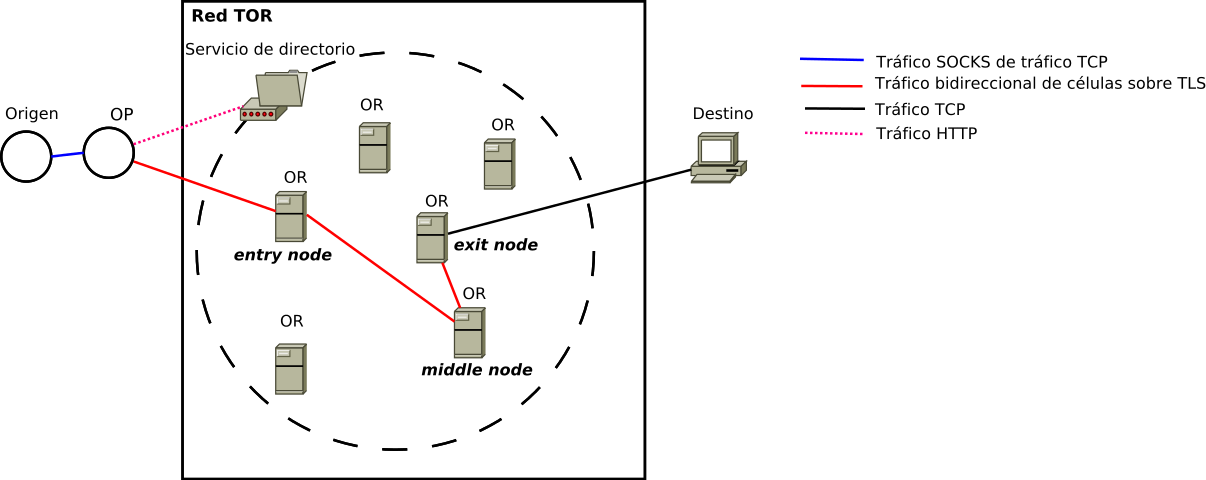
\includegraphics[width=\textwidth]{imagenes/funcionamiento_tor}
	\caption{Funcionamiento de la red Tor.}
	\caption*{\small \url {https://es.wikipedia.org/wiki/Tor_(red_de_anonimato)}}
	\label{fig:redtor}
\end{figure}

\subsubsection {Hidden Services}

Los hidden services son, como su nombre indica, servicios alojados en la red TOR que se comunican con sus usuarios de forma exclusiva por medio de la misma. El dominio para acceder a los hidden services se trata de un hash de 16 caracteres derivado de su clave privada y acabado en ``.onion". \\

Los usuarios hacen uso de los \hyphenquote{spanish}{rendezvous points} ó puntos de encuentro (OR que actúan como tales), para conectarse con los hidden services. Es en este punto donde se realiza el intercambio de claves entre usuario y servicio, con el punto de encuentro como intermediario y mediador en la comunicación. \\ 


\subsubsection {Tipos de Nodos}

\textbf {Onion Router (OR)} \\
Entidades clave en la arquitectura de la red, una de sus funciones es enrutar el tráfico a través de la red y actuar como servidores de directorios para la comunicación de los usuarios con hidden services. Los servidores de directorios son OR con operadores de confianza, encargados de mantener y difundir la base de datos con la información de otros OR. \\

Cuando un OR se conecta a la red, se define a sí mismo compartiendo y exponiendo su funcionamiento y capacidades (versión, banda ancha, política de enrutamiento, etc). \\

\textbf {Onion Proxy (OP)} \\
Se trata de la entidad que representa el software ejecutado por el usuario. Obtiene además información acerca del estado de la red y realiza el cálculo del camino aleatorio de la comunicación. De forma que pueda cumplir su función de enrutar el tráfico TCP hacia TOR.

\subsubsection {Funcionamiento}

Las aplicaciones que deseen comunicarse mediante TOR pueden hacerlo siguiendo la interfaz SOCKS, la cual actúa como intermediaria entre la aplicación y la red. \\

Una vez conectado a la red, el usuario solicita a un servicio de directorio información sobre la red (Nodos OR), y decide un camino aleatorio para los paquetes. Este camino consta de un nodo de entrada, un nodo intermedio y un nodo de salida. \\

El camino de la comunicación se genera de forma sucesiva: primero generando las claves de cifrado, posteriormente aplicando un Diffie-Hellman\cite{WikiDiffieHellman} entre los puntos a comunicarse y por último el envío de las claves y comunicación cifrada mediante RSA (claves pública y privada). \\

%TODO: Referencias a Diffie-Helman y a RSA.

Una vez que las claves RSA han sido establecidas, este es considerado como un medio seguro para la comunicación, y se procede al envío de los paquetes que irán encapsulados en capas de cifrado que se podrán romper a cada salto hasta llegar al destino. \\ 

%TODO: Refrasear lo ultimo, lo de los saltos.

\begin{figure}[H]
	\centering
	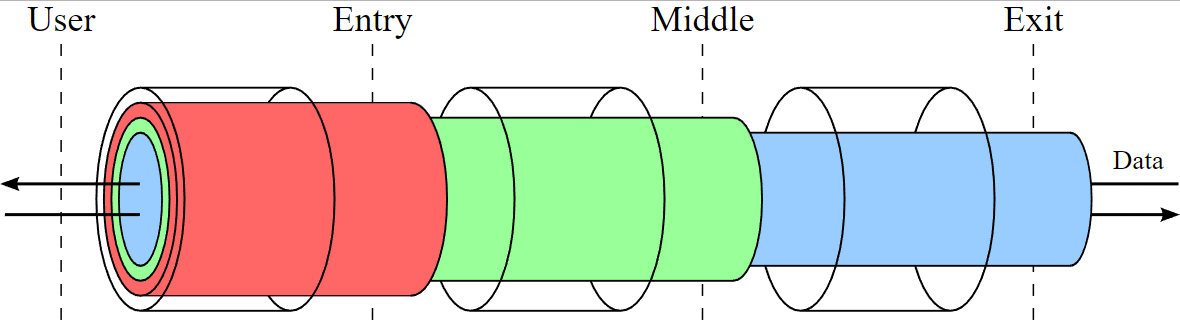
\includegraphics[width=\textwidth]{imagenes/tor_keys}
	\caption{Funcionamiento de la red Tor.}
	\caption*{\small \url {https://svn.torproject.org/svn/projects/presentations/security-part2-anon/}}
	\label{fig:torkeys}
\end{figure}

\subsubsection {Puntos flacos}

Pese a disponer de un extenso equipo de expertos desarrolladores y criptógrafos, TOR está sujeto a una constante caza de vulnerabilidades y búsqueda de métodos para romper la protección que brinda a los usuarios. \\
Los principales interesados en conseguirlo son entidades gubernamentales y servicios de inteligencia de diversos países, que pese a esto, son también usuarios de primera mano de TOR y sus servicios. \\ 

Los principales ataques se basan en la correlación de tiempos de envío y tamaños de paquetes en la red, los cuales mediante una análisis sistemático y controlando un relativamente grande numero de nodos, permitirían destapar la identidad de los usuarios. \\

Desde un punto de vista de usuario, la principal desventaja de TOR se halla en que por diseño, su característica es la protección de la identidad de la cual proviene la información, pero no la ofuscación o privacidad de la misma. Es decir, pese a usarse la red TOR para acceder a un servicio, si la comunicación se realiza en texto plano, cualquier tercero escuchando tanto en la entrada o salida de la red podrá interceptar las comunicaciones. \\ 

Los puntos principales que podrían comprometer nuestra identidad durante su uso son los siguientes: \\

\begin{itemize}  
	\item  Código Javascript malicioso
	\item  Cookies
	\item  Cabeceras HTTP
	\item  Uso de HTTP en lugar de HTTPS
	\item Peticiones DNS no redireccionadas por TOR
	\item  Plugins (Java, Flash, etc)
\end{itemize}

\subsection {Node.js}

Node.js es un interprete de JavaScript desarrollado sobre el motor V8 de Chrome, de forma que extiende el uso del lenguaje también en el lado del servidor. Consta además, de uno de los ecosistemas de librerías más grandes en existencia. \\

Pese a disponer de una librería para el manejo de operaciones sobre HTTP, es también gracias a paquetes como Express o Hapi que Node.js se ha extendido en gran medida como herramienta para desarrollar servidores y aplicaciones web. \\
El modelo de Node.js esta basado en eventos y operaciones de E/S no bloqueantes, lo que lo hace eficiente en el tratamiento de peticiones concurrentes.

\subsection {Websockets}

Websocket es un protocolo que proporciona un canal de comunicación bidireccional entre cliente y servidor sobre un mismo socket TCP. \\

El uso de sesiones de este tipo es especialmente útil en aplicaciones donde es ventajoso que el servidor pueda enviar datos también al cliente; siendo este caso imposible en las formas de comunicación convencionales entre cliente y servidor como XHR (AJAX), donde es el cliente el encargado de iniciar cada intercambio de información. \\

El protocolo de websockets consta de soporte en las versiones más modernas de casi todos los navegadores. Sin embargo, puede no ser viable su uso en versiones más antiguas. Para solventar este problema, se ha hecho uso de la librería Socket.io de Node.js. \\

Socket.io implementa una interfaz para la comunicación sobre websockets con un mecanismo para pivotar hacia otros modelos de comunicación en caso de que el medio no conste de soporte para estos. \\
\subsection {Electron}

Electron es una librería desarrollada por Github que permite crear aplicaciones de escritorio multiplataforma mediante Javascript, CSS y HTML. \\
Ésto se consigue combinando Node.js y Chromium (navegador de código libre sobre el que está basado Chrome). De esta forma se crea un entorno de ejecución con funcionalidades cliente-servidor. \\

Una de las principales aplicaciones desarrolladas con Electron es Atom, el editor de texto de código libre desarrollado por Github. Sin embargo, hay multitud de aplicaciones utilizadas por millones de usuarios que se apoyan en esta tecnología, entre ellas encontramos Slack, Visual Studio Code, Wordpress.com y Discord, entre otras. \\

\subsection {React}

React es una librería desarrollada por Facebook para la creación de interfaces de usuario basadas en componentes. \\

Hace uso de JSX, una sintaxis extendida de Javascript que permite la declaración de etiquetas HTML junto con variables y funciones, además de otras características. \\

Los componentes se suelen organizar de forma jerárquica, donde la información fluye del componente padre a sus hijos, en forma de propiedades (props). Los componentes hijos tienen la capacidad de notificar al padre de una acción de usuario o un cambio de estado mediante llamadas a funciones (recibidas en forma de props).\\

\subsubsection {Componentes, estado, propiedades y renderizado}

Los componentes constan de estado, propiedades y ciclo de vida. El estado son las características propias del componente, mientras que las propiedades son aquellos valores recibidos externamente, normalmente por el componente padre. Al cargarse la vista, estos se renderizan, y conforme el estado se modifica por acciones del usuario o las propiedades recibidas cambian, estos avanzan por las distintas etapas del ciclo de vida y vuelven a renderizarse. \\

\subsubsection {DOM Virtual}

React genera un DOM virtual sobre el que se construyen los componentes. Después de una actualización del estado se compara el DOM anterior con el actual, actualizando y modificando de forma eficiente la vista, ya que solo se renderizan de nuevo aquellas partes necesarias.  \\

\subsubsection {Multiplataforma}

Facebook ha desarrollado también una adaptación de React para plataformas móviles, llamada React Native.

\subsection {React Native} 

Ésta funciona con los mismos principios que React y también se desarrolla mediante Javascript, pero utilizando en el renderizado componentes propios de la librería en lugar de etiquetas HTML, que posteriormente se traducen a componentes nativos. De esta forma es posible creat una aplicación móvil nativa y con todas las propiedades de las mismas. \\

\subsection {Redux}

Redux es una librería de Javascript, que aunque agnóstica, ha sido desarrollada con su uso combinado con React en mente. \\ 

Redux permite mantener un estado central de la aplicación como única fuente de verdad e implementa un flujo de información unidireccional, que resulta muy ventajoso en aplicaciones grandes y/o complejas. \\

El proceso de actualización de estado en Redux es el siguiente: 

\begin{enumerate}  
	\item  Un evento, por ejemplo la interacción del usuario, produce un cambio en la vista.
	\item Se despacha una acción asociada a ese evento. 
	\item La acción es procesada por un reducer, que se encarga de interpretar esa acción y aplicar el cambio sobre la Store, o el estado central de la aplicación, conforme corresponda.
\end{enumerate}

Para operaciones asíncronas, como llamadas a APIs o eventos similares, Redux puede emplearse con middlewares que extienden su funcionalidad. Para este caso tenemos \hyphenquote{spanish}{redux-thunk}, que permite declarar acciones más allá de simple objectos Javascript, y declararlas como funciones. De esta manera pueden lanzarse diversas acciones dependiendo del estado de la petición o la operación, manteniendo la Store actualizada en todo momento. \\

Las acciones se ejecutan de forma secuencial, evitando de esta manera condiciones de carrera o estados inconsistentes de los datos. \\

\subsubsection {Estado inmutable}

La Store, o el estado de la aplicación, se trata de un objeto que contiene toda la información referente a esta y se trata de forma inmutable. O lo que es lo mismo, cuando se debe actualizar el estado de la aplicación debido a una acción, los reducers crean una copia del estado anterior modificado, y este substituye al estado anterior. Esto resulta de especialmente eficiente cuando se deben tratar gran cantidad de datos con cambios constantes o sistemáticos. Resulta mucho más rápido que la comparación en más profundidad. \\

Para realizar estas operaciones se hace uso de librerias que tratan los objectos como inmutables, de la función Object.assign(...) ó si se dispone de la versión de Javascript ES6 en el proyecto, el operador spread. \\


\chapter{Estado del arte}

Pese a que en los pasados años ha habido una creciente tendencia en la adopción de tecnologías de cifrado punto a punto en las aplicaciones de mensajería comerciales, esto no significa directamente que los usuarios estén mejor protegidos o que los datos de las conversaciones privadas se traten de una forma más segura. \\

Esto es debido a que aunque muchos servicios tienen la opción de activar el cifrado punto a punto, impidiendo al servidor intermedio, es decir, al proveedor del servicio (Facebook, Google, etc), interceptar y analizar el contenido, la mayoría de estos no lo tienen como opción activada por defecto. Por lo tanto, el usuario ha de buscar y activar expresamente las funciones relacionadas con aumentar la seguridad, generalmente  denominadas como \hyphenquote{spanish}{conversaciones secretas}, para que estas características se hagan efectivas. \\

A continuación se ha realizado un análisis de las aplicaciones más populares de mensajería y una consideración de sus características de seguridad, así como de la usabilidad o facilidad de acceso de los usuarios a las mismas. Se ha dedicado un apartado individualmente a cada una de las aplicaciones más relevantes, haciendo hincapié en los pros y contras que presentan respecto a sus competidores. \\

\pagebreak

\section {Comparativa}

\begin{table}[h]
	\centering
	\label{comparativa-applicationes-mensajeria}
	\resizebox{\textwidth}{!}{%
		\begin{tabular}{|c|c|c|c|c|}
			\hline
			& \textbf{WhatsApp} & \textbf{Facebook Messenger} & \textbf{Telegram} & \textbf{Signal} \\ \hline
			Cifrado punto a punto                                                                                                 & Sí                & Sí                          & Sí                & Sí              \\ \hline
			\begin{tabular}[c]{@{}c@{}}Cifrado punto a punto \\ activado por defecto\end{tabular}                                 & Sí                & \textcolor{red}{No}                          & \textcolor{red}{No}                & Sí              \\ \hline
			\begin{tabular}[c]{@{}c@{}}Implicado en compartir\\ datos con agencias de inteligencia\end{tabular} & Sí                & Sí                          & \textcolor{red}{No}                & \textcolor{red}{No}              \\ \hline
			\begin{tabular}[c]{@{}c@{}}Compañía colecciona \\ datos de usuarios\end{tabular}                                      & Sí                & Sí                          & Sí                & \textcolor{red}{No}              \\ \hline
			Totalmente código abierto                                                                                             & \textcolor{red}{No}                & \textcolor{red}{No}                          & \textcolor{red}{No}                & Sí              \\ \hline
			\begin{tabular}[c]{@{}c@{}}Claves de cifrado generadas\\  en el dispositivo\end{tabular}                              & Sí                & Sí                          & Sí                & Sí              \\ \hline
			\begin{tabular}[c]{@{}c@{}}Mensajes cifrados \\ con claves individuales\end{tabular}                                  & Sí                & Sí                          & \textcolor{red}{No}                & Sí              \\ \hline
			\begin{tabular}[c]{@{}c@{}}Se almacenan tiempos de envío\\ y/o IPs\end{tabular}                                       & Sí                & Sí                          & Sí                & \textcolor{red}{No}              \\ \hline
			\begin{tabular}[c]{@{}c@{}}Reciente auditoría \\ de código y/o protocolo\end{tabular}                                 & \textcolor{red}{No}                & \textcolor{red}{No}                          & Sí                & Sí              \\ \hline
			Posibilidad de registro anónimo                                                                                       & \textcolor{red}{No}                & \textcolor{red}{No}                          & \textcolor{red}{No}                & \textcolor{red}{No}              \\ \hline
			\begin{tabular}[c]{@{}c@{}}Compañía puede leer\\ contenido de mensajes\end{tabular}                                   & \textcolor{red}{No}                & Sí                          & Sí                & \textcolor{red}{No}              \\ \hline
		\end{tabular}%
	}
\end{table}

\subsubsection {WhatsApp}

Con aproximadamente mil trescientos millones de usuarios diarios (Julio 2017), WhatsApp cuenta con la corona en el mercado de aplicaciones de mensajería. \\

%TODO: Reference a lo de los usuarios diarios.

Fue fundada en 2009 por Jan Koum y gracias a la adopción de internet en los dispositivos móviles y la ubiquidad de los mismos, ha crecido exponencialmente desde entonces. Su rápida adopción fue también debido a la enorme ventaja contra los SMS, que contaban con un límite de caracteres y su coste de uso era mucho mayor. \\

En febrero de 2014 Facebook anunció su compra, y finalmente fue adquirida por 21.800 millones de dólares. \\

Gracias a una colaboración con \hyphenquote{spanish}{Open Whispers}, a día de hoy cuenta con la integración del protocolo Signal en todas sus comunicacione: mensajes de texto, voz y videollamadas. Todas sus formas de comunicación vienen cifradas punto a punto por defecto y de forma transparente al usuario. \\

A efectos prácticos, WhatsApp protege a sus usuarios de espías intermedios y ni ellos mismos son capaces de leer el contenido de las comunicaciones en sus servidores. \\

%TODO: Referencia a lo que es Open Whispers.

Sin embargo, WhatsApp sí que almacena los tiempos de envío de los mensajes, así como identidad del emisor y receptor de los mismos; entre otra tanta información catalogada como \hyphenquote{spanish}{metadatos}. \\

Dichos metadatos pueden definirse de forma certera como la información referente a la actividad. Es decir, no se trata del contenido propiamente dicho, si no de la información respecto a la naturaleza del mismo. Por lo tanto, en esta categoría entran aspectos como: información respecto al dispositivo, posición GPS, contactos, horas de conexión, conexiones inalámbricas, duración de las comunicaciones, tamaño de los paquetes enviados, etc. \\

Por otro lado, Facebook fue mencionado en los documentos filtrados por Edward Snowden en 2013 como una de las compañías que cedía el acceso a los datos de sus usuarios a la agencia de seguridad nacional de EE.UU. (NSA). \\

En conclusión, WhatsApp se presenta como una herramienta de comunicación que cuenta con la tecnología y las herramientas adecuadas pero implementadas de forma que no se cubren completamente los aspectos necesarios para garantizar una privacidad absoluta de sus usuarios, así como la protección de los mismos frente a un escrutinio por parte de un adversario como una entidad gubernamental. \\

\subsubsection {Facebook Messenger}

Facebook Messenger es la aplicación de mensajería que acompaña a la aplicación móvil de la red social. \\

Fue lanzada en 2004 bajo el nombre de Facebook Chat, y desde entonces ha sido adoptada por una enorme cantidad de usuarios. Uno de los posibles motivos de esta acogida puede ser el hecho de que Facebook la ha convertido en un requisito para establecer comunicaciones en la red social, de forma que es imposible continuar con la misma experiencia de uso en Facebook sin descargarla e instalarla. \\

Como se ha mencionado anteriormente en la tabla comparativa, Facebook Messenger dispone de cifrado punto a punto en forma de chats secretos, que no están habilitados por defecto. En su uso normal, la aplicación solamente cifra el tráfico entre los usuarios y sus servidores. Es decir, la empresa es capaz de leer el contenido de las comunicaciones (tanto texto como contenido multimedia). \\

Facebook Messenger es un claro ejemplo de la adopción de una tecnología que debería ser ubicua en todas las comunicaciones modernas, pero implementada con lo que parece ser una motivación puramente comercial, ya que la enorme mayoría de usuarios no conoce la existencia de esta característica; y de entre los que la conocen, son aún menos los que la utilizan.

\subsubsection {Telegram}

Telegram es una aplicación de mensajería fundada y desarrollada en 2013 por los hermanos Nikolai y Pavel Durov. \\

Pavel Durov es un conocido emprendedor y millonario de origen ruso, famoso por ser el fundador de la red social VK. Nikolai, por otra parte, fue CTO de la anterior mencionada red social, y cuenta con una extensa formación académica tanto en matemáticas como en informática; ha obtenido, además, diversas medallas y condecoraciones en olimpiadas y competiciones en ambos campos. \\

El protocolo de Telegram, MTProto, fue desarrollado desde cero por Nikolai, lo cual ha ocasionado diversas dudas respecto a su seguridad y fiabilidad para un uso en producción en la escala de Telegram. \\

Por otro lado, pese a disponer de la opción de chats secretos cifrados punto a punto, estos no se encuentran activados por defecto. En consecuencia, las conversaciones pueden ser leídas y el contenido visualizado en los servidores de la compañía sin ningún impedimento. \\

La función de chat privados hace uso de un cifrado punto a punto donde las claves generadas en el dispositivo son reutilizadas múltiples veces, por lo que se pierde la característica denominada como \hyphenquote{spanish}{forward secrecy}. Si se logra acceder a las claves de cifrado, todos los mensajes serán accesibles para el atacante. Por otro lado, la opción de chats secretos no se encuentra disponible actualmente para las versiones de escritorio de la aplicación. \\

Telegram, pese a ser un legítimo rival para WhatsApp en cuanto a funcionalidad, carece de una base criptográfica sólida.

\subsubsection {Signal}

Signal es una aplicación de mensajería de código libre, enfocada en la seguridad y privacidad de sus usuarios. Fue creada en 2014 por Open Whispers Systems (OWS), la misma organización que originó el protocolo del mismo nombre. Fue cofundada por Moxie Marlinspike, coautor de las bases criptográficas del protocolo Signal. Signal es en la actualidad uno de los sistemas de comunicación más seguros. Tiene origen en la fusión de dos proyectos previos, TextSecure y RedPhone, ambas lanzadas por OWS en 2010. Signal destaca en buenas prácticas de seguridad, criptografía y trato de datos de usuarios. \\

Todas las comunicaciones están cifradas punto a punto, incluidos los metadatos referentes a las mismas. El almacenamiento de información de usuario se ha reducido al mínimo indispensable para mantener la plataforma, y toda la información restante resulta cifrada de forma que nadie más que los usuarios puede acceder a ella. Las claves de cifrado son generadas en los dispositivos, no compartidas en ninguna otra parte, y las claves utilizadas son únicas en cada mensaje, de forma que la pérdida o filtrado de las mismas no implica el acceso a mensajes previos. Signal implementa, además, formas de comprobar la identidad del usuario con el que nos estamos comunicando, así como métodos para detectar una suplantación de identidad. \\

También se han realizado diversos estudios de cara a su usabilidad y accesibilidad por parte de los usuarios menos versados al buen uso de sus características de seguridad; por desgracia, los estudios demostraron que los usuarios tenían dificultades para identificar una suplantación de identidad, aunque los esfuerzos en la mejora de la interfaz y usabilidad han incrementado. \\

Su base criptográfica ha recibido frecuentes revisiones por diversos expertos y equipos a lo largo del planeta, siendo además su código completamente libre y abierto al escrutinio de la comunidad. \\

El uso de Signal como medio de comunicación es predicado por expertos en criptografía, seguridad y vigilancia de la talla de Edward Snowden (Ex-CIA, Ex-NSA), Bruce Schneier (junta directiva de la EFF, experto criptógrafo, autor) o Isis Agora Lovecruft (desarrolladora líder en TOR). \\

\chapter{Servicio de mensajería: privado y anónimo}

El trabajo sobre el cual se basa esta memoria consiste en el desarrollo de un sistema de mensajería que implemente funcionalidades que protejan tanto la identidad como la privacidad de sus usuarios. Para ello, la intención ha sido mezclar las dos tecnologías estado del arte en ambos panoramas, el protocolo Signal y el protocolo TOR. \\

El servidor se ha desarrollado en Node.js, haciendo uso de la librería para el manejo de websockets Socket.io. \\

Por otro lado, el cliente de escritorio hace uso de la librería Electron, de la cual se obtiene una base para un desarrollo sencillo multiplataforma. Se ha hecho uso también del framework React junto con Redux, para implementar la lógica de la vista de usuario y manejar las conexiones. \\

Además, se ha implementado a modo de experimento una versión del sistema para la mensajería en dispositivos móviles, aunque este carece de la funcionalidad de cifrado y ofuscación de identidad. Para este fin se ha hecho uso de la tecnología React Native. \\

El protocolo Signal se ha implementado mediante el uso de la librería creada por la organización Open Whispers Systems para el desarrollo de proyectos en Javascript. \\

En cuanto a la inclusión de TOR en la comunicación de la plataforma, se ha creado un hidden service (servicio en la red TOR), y se ha trabajado de cara a la conexión a través de esta red. Un requerimiento para conseguir tal conexión es entablar comunicación mediante el protocolo SOCKS, para el cual no existe actualmente adaptación por parte de la librería de websockets utilizada. A pesar de invertir una cantidad considerable de tiempo y esfuerzo en su inclusión, no ha sido posible implementar la comunicación a través de dicha red. Queda pues como una característica a implementar en el futuro, en la que se trabajará fuera del marco del trabajo de fin de grado. \\ 


\chapter{Planificación}

\section{Historias de usuario}

Se ha abordado la planificación del proyecto siguiendo metodologías ágiles, con historias de usuario definiendo la funcionalidad necesaria a implementar desde el punto de vista del usuario, y además, iterando sobre las tareas desde implementaciones básicas, pero funcionales, hasta conformar las más complejas y completas. \\ 

Se ha planificado el desarrollo en tres grandes hitos:

\begin{enumerate}
	\item \textbf{Servicio de mensajería}
	\item \textbf{Uso del protocolo Signal}
	\item \textbf{Despliegue de la aplicación en la red TOR}
\end{enumerate}

Se han conseguido realizar únicamente dos de tres de estos hitos planteados inicialmente; el último de ellos no ha sido completado pero se ha realizado una investigación referente a la tecnología, el funcionamiento y las posibilidades de implementación de la solución al hito. \\ 

A continuación se detallan, agrupadas por hitos, las distintas tareas realizadas: \\ 


\subsection{Hito 1: Sistema de mensajería}
\begin{adjustbox}{margin=2.5ex 5ex 2.5ex 2.5ex,center}
	\begin{forest} for tree={
	    growth parent anchor=south,
	    parent anchor=south,
	    child anchor=north,
	    edge path={none}, 
	    l sep=.25cm,
	}   
	%
	[Sistema de mensajería, goal, name=agoal
	    [Cliente, activity
	        [1. Conexión básica con el servidor, task
	       	[2. Mostrar mensaje de bienvenida{,} logo y login, task
	        [3. Mostrar usuarios conectados, task
	        [4. Iniciar conversación con un usuario, task
			[5. Mostrar usuario en la barra de navegación durante conversación, task
			[6. Recibir mensajes enviados al usuario cuando éste se encuentra desconectado, task			
	        [7. Link para volver a la lista de usuarios desde la conversación, task
	        [8. Actualizar estado de usuarios en tiempo real cuando estos se conectan/desconectan, task
	        [9. Mejora de estilos de vista\, presentación y efectos visuales, task	        
	        [9. Conectar con servidor desplegado, task	  	        
	        ] ] ] ] ] ] ] ] ] ] ]
	    [Servidor, activity
	        [1. Conexión básica con los clientes, task
			[2. Permitir registro de usuarios en la aplicación mediante nombre, task
	        [3. Enviar información respecto a usuarios conectados a los clientes, task
	        [4. Redirigir mensajes entre clientes en las conversaciones, task
	        [5. Almacenar mensajes cuando los usuarios están desconectados\, enviarlos cuando se conectan, task
	        [6. Enviar actualizaciones de usuarios conectados/desconectados en tiempo real a los clientes, task
 	        [6. Desplegar en una máquina servidor, task
	        ] ] ] ] ] ] ] ] ]
	%           
	\end{forest}
\end{adjustbox}

Una vez alcanzado este hito, la funcionalidad del proyecto cubre las necesidades básicas para mantener un sistema de chat entre múltiples usuarios en tiempo real. Esto supone la base sobre la que se implementarán las medidas de cifrado y seguridad.
	
\subsection{Hito 2: Uso del protocolo Signal}

\begin{adjustbox}{margin=2.5ex 5ex 2.5ex 2.5ex,center}
	\begin{forest} for tree={
			growth parent anchor=south,
			parent anchor=south,
			child anchor=north,
			edge path={none}, 
			l sep=.25cm,
	}   
	%
	[Uso del protocolo Signal, goal, name=bgoal
		[Cliente, activity
		[1. Generación de claves de cifrado al iniciar la aplicación, task
		[2. Solicitar y proveer claves al servidor según sea necesario durante la conversación, task
		[3. Cargar sesión con el usuario con el que se desee establecer una conversación, task
		[4. Descifrar mensajes entrantes usando claves de cifrado del usuario con el que se conversa, task
		[5. Cifrar mensajes al enviarlos{,} en el formato adecuado, task] ] ] ] ] ]
		[Servidor, activity
		[1. Redirigir peticiones y respuestas a peticiones de claves, task] ] ] 
	%           
	\end{forest}
\end{adjustbox}

En este hito se ha pretendido implementar la funcionalidad básica de cifrado del protocolo Signal, generando claves para cada mensaje intercambiado. \\

Una nueva clave publica es derivada de la clave privada de los usuarios a cada mensaje que se desea enviar, y se comprueba la validez de los mensajes mediante la firma de los mismos con la clave de identidad de cada usuario.
El servidor se trata finalmente como una entidad en la que no se confía, y la información que pasa a través del mismo no es accesible en texto plano. \\

Una vez implementado este punto, damos por implementada la funcionalidad que trata de preservar la privacidad en la comunicación. \\ 

\subsection{Hito 3: Despliegue en la red Tor}
\begin{adjustbox}{margin=2.5ex 5ex 2.5ex 2.5ex,center}
	\begin{forest} for tree={
			growth parent anchor=south,
			parent anchor=south,
			child anchor=north,
			edge path={none}, 
			l sep=.25cm,
	}   
	%
	[Despliegue en la red Tor, goal, name=cgoal
		[Cliente, activity
		[Conectar al servidor mediante la red TOR, task] ]
		[Servidor, activity
		[Deplegar servidor como hidden service, task
		[Conectar clientes a través de la red TOR, task ] ] ] ] 
	%           
	\end{forest}
\end{adjustbox}

En este hito se pretende cubrir el aspecto de la protección de la identidad de los usuarios, mediante la conexión a través de la red TOR. Así como de la ofuscación del servidor, desplegándolo como hidden service \cite{HiddenServiceTorProject} en la misma red. \\

\section{Diagrama de componentes}

\begin{figure}[H]
	\centering
	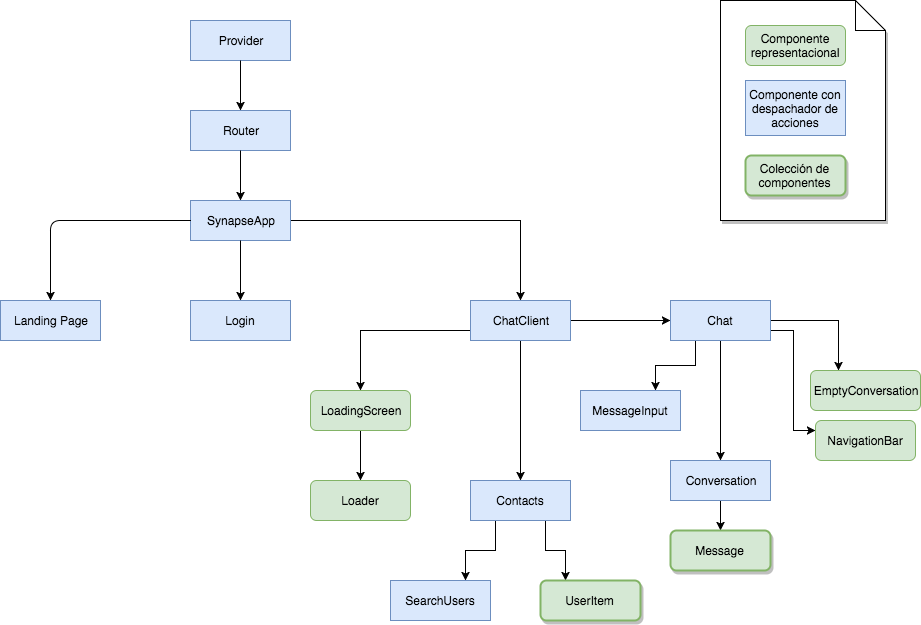
\includegraphics[width=\textwidth]{imagenes/diagrama-componentes}
	\caption{Diagrama de componentes}
	\label{fig:diagrama-componentes}
\end{figure}

Las aplicaciones React se estructuran en componentes ordenados en una jerarquía padre-hijo, donde los hijos reciben propiedades (props) del padre, y notifican a este de cambios en el estado según la interacción del usuario a través de llamadas a funciones, también recibidas por el mismo mecanismo que las propiedades.\\ 

Debido a esta naturaleza de React no se ha realizado un diagrama de clases UML. Sino que se ha realizado un diagrama donde se representan estas relaciones padre-hijo entre componentes y se hace distinción entre aquellos puramente representacionales (sin lógica) y aquellos que despachan acciones. \\ 
\chapter{Implementación}

Como se ha mencionado anteriormente en la descripción de la aplicación, esta se encuentra dividida en dos partes fundamentales: El cliente y el servidor. \\
Para alojar el código del proyecto, se ha creado una organización en Github: SynapseMessenger; bajo la cual se han creado los repositorios pertenecientes a los distintos aspectos del proyecto: Servidor, Cliente de escritorio, cliente de móvil y documentación. \\ 
\chapter{Conclusiones y trabajos futuros}

Los recursos necesarios para desarrollar la aplicación se han encontrado en sitios web de libre acceso, el software propio de las librerías utilizadas referentes a los protocolos de comunicación y cifrado es de carácter libre y consta de licencias de código abierto. \\

En dicho sentido, el objetivo principal de desarrollo se ha alcanzado, puesto que se ha comprobado la posibilidad del desarrollo de una aplicación que provea un medio de comunicación libre, seguro, privado y anónimo. \\ 

Esta última característica no se ha conseguido implementar, por una parte debido a la falta de adaptación de la librería de websockets elegida, y por otra, por la diferencia que supone el desarrollo de una aplicación de escritorio en Electron a un agente de navegador web convencional. La adaptación a la interfaz SOCKS podría haberse realizado de disponer de un cliente de navegador y más tiempo para el desarrollo; este es el principal punto a recalcar como trabajo futuro. \\

Por otro lado, la funcionalidad referente a los mensajes pendientes se ha tenido que eliminar en pos de la implementación del cifrado Signal. Hubiera sido posible implementar un sistema de cero confianza en el servidor con mensajes pendientes, pero éstos tendrían que haber reutilizado claves de cifrado, en lugar de claves efímeras en cada mensaje. Otra posibilidad hubiese sido establecer una clave de cifrado para mensajes pendientes entre ambos usuarios. \\

La intención es continuar el trabajo de la aplicación más allá del alcance de este trabajo de fin de grado, implementando métodos para verificar la identidad de los usuarios y conversaciones en grupo. \\

%
\nocite{*}
\bibliography{bibliografia}\addcontentsline{toc}{chapter}{Bibliografía}
\bibliographystyle{unsrt}
%
%\appendix
%\input{apendices/manual_usuario/manual_usuario}
%%\input{apendices/paper/paper}
%\input{glosario/entradas_glosario}
% \addcontentsline{toc}{chapter}{Glosario}
% \printglossary
\chapter*{}
\thispagestyle{empty}

\end{document}
